\chapter[Simulatie resultaten]{Simulaties resultaten van de controller}
\label{Ap:sim_controller}
\section{Behavioral simulatie}
\begin{figure}[ht!]
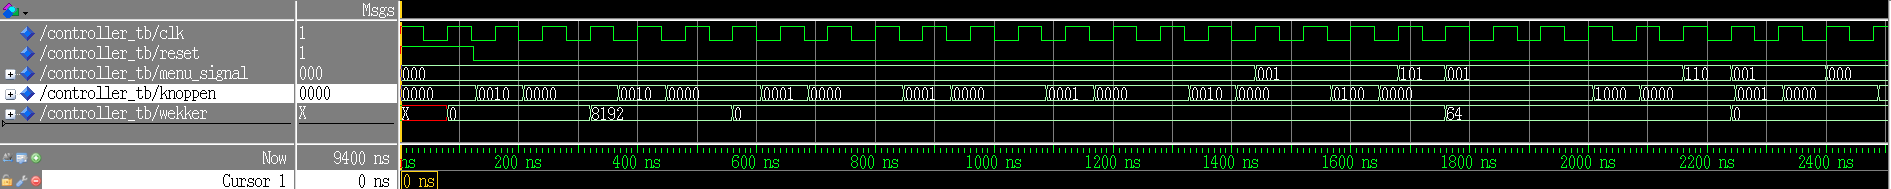
\includegraphics[width=\textwidth,height=\textheight,keepaspectratio]{Figuren/Controller/wave0-2_5.png}
\caption{Simulatie van 0 tot 2500ns}
\label{fig:sim_beh_0-2_5}
\end{figure}
\begin{figure}[ht!]
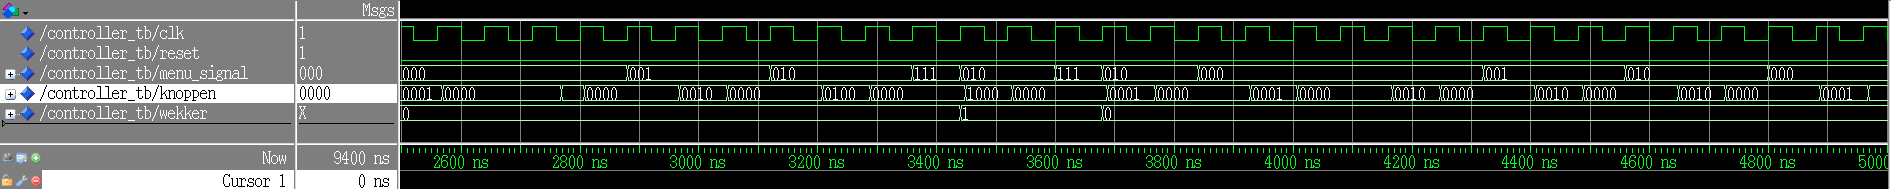
\includegraphics[width=\textwidth,height=\textheight,keepaspectratio]{Figuren/Controller/wave2_5-5.png}
\caption{Simulatie van 2500ns tot 5000ns}
\label{fig:sim_beh_2_5-5}
\end{figure}
\begin{figure}[ht!]
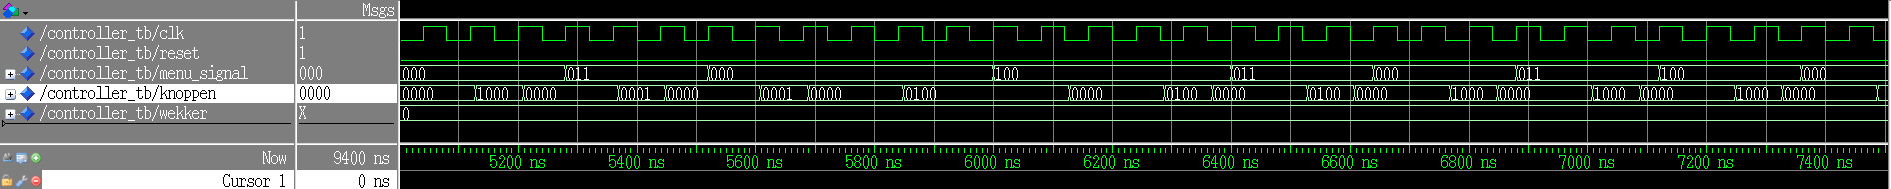
\includegraphics[width=\textwidth,height=\textheight,keepaspectratio]{Figuren/Controller/wave5-7_5.png}
\caption{Simulatie van 5000ns tot 7500ns}
\label{fig:sim_beh_5-7_5}
\end{figure}
\begin{figure}[ht!]
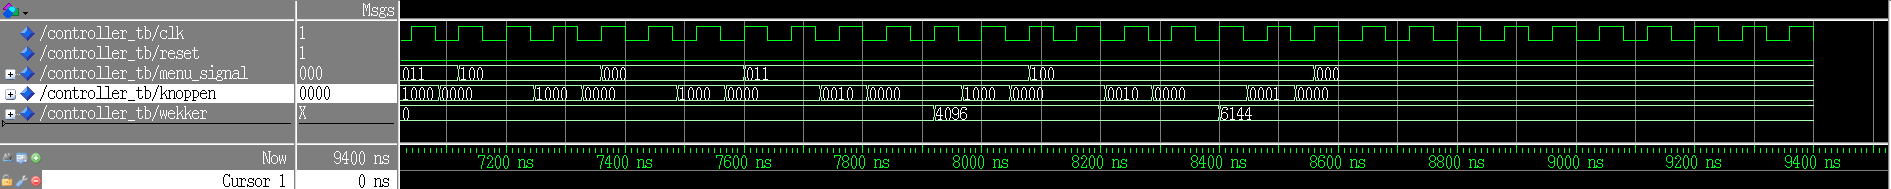
\includegraphics[width=\textwidth,height=\textheight,keepaspectratio]{Figuren/Controller/wave7_5-.png}
\caption{Simulatie van 7500ns tot het einde}
\label{fig:sim_beh_7_5-}
\end{figure}
\newpage
\section{Synthesize simulatie}
\begin{figure}[ht!]
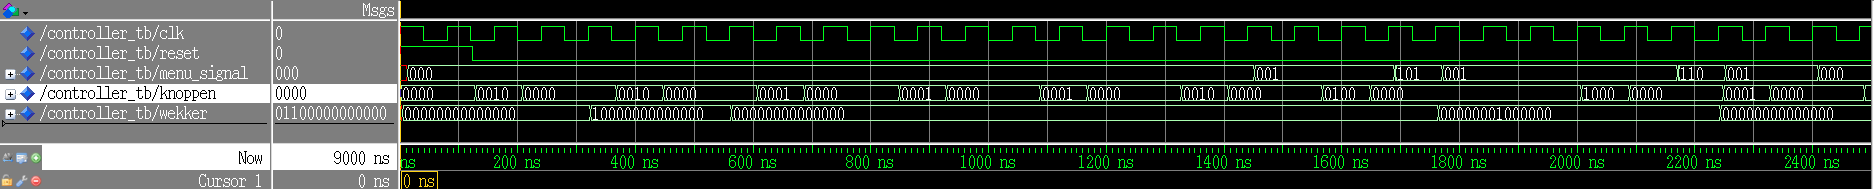
\includegraphics[width=\textwidth,height=\textheight,keepaspectratio]{Figuren/Controller/wave0-2_5_syn.png}
\caption{Simulatie van 0 tot 2500ns}
\label{fig:sim_syn_0-2_5}
\end{figure}
\begin{figure}[ht!]
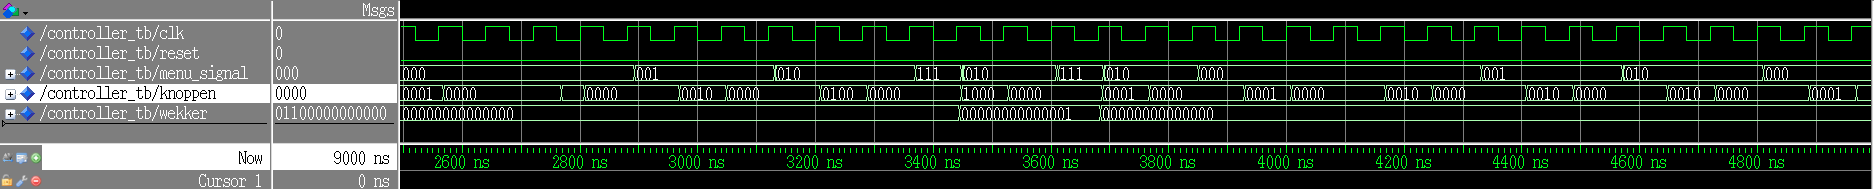
\includegraphics[width=\textwidth,height=\textheight,keepaspectratio]{Figuren/Controller/wave2_5-5_syn.png}
\caption{Simulatie van 2500ns tot 5000ns}
\label{fig:sim_syn_2_5-5}
\end{figure}
\begin{figure}[ht!]
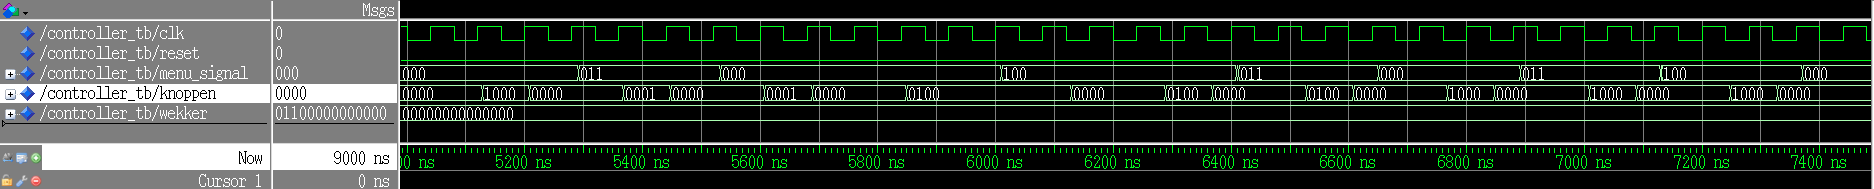
\includegraphics[width=\textwidth,height=\textheight,keepaspectratio]{Figuren/Controller/wave5-7_5_syn.png}
\caption{Simulatie van 5000ns tot 7500ns}
\label{fig:sim_syn_5-7_5}
\end{figure}
\begin{figure}[ht!]
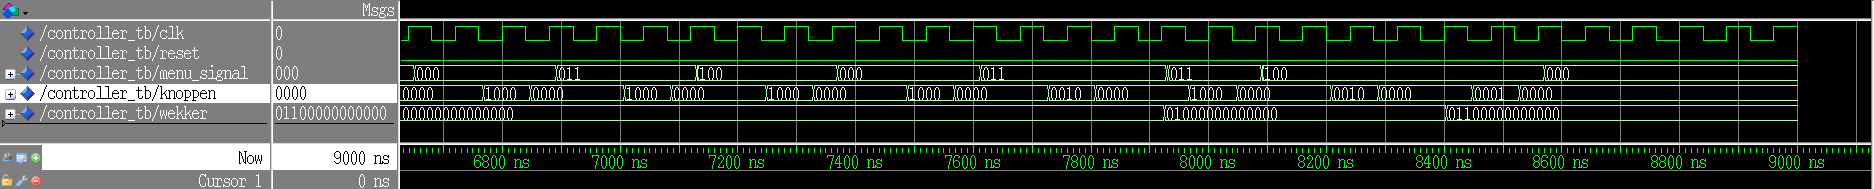
\includegraphics[width=\textwidth,height=\textheight,keepaspectratio]{Figuren/Controller/wave7_5-_syn.png}
\caption{Simulatie van 7500ns tot het einde}
\label{fig:sim_syn_7_5-}
\end{figure}
\newpage
\section{Extracted simulatie}
\begin{figure}[ht!]
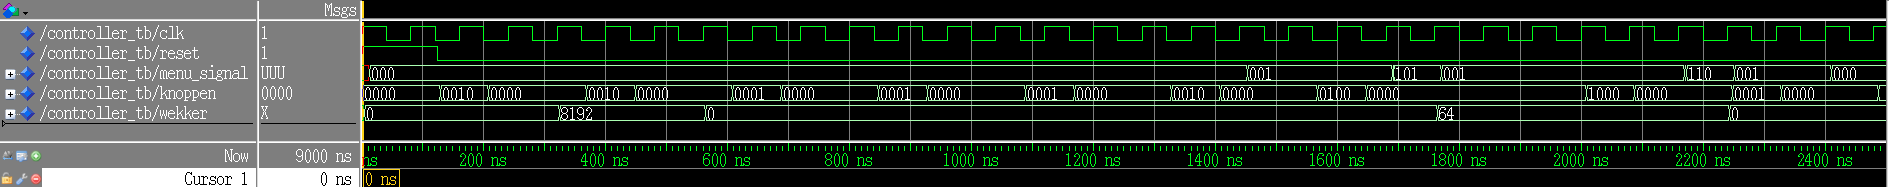
\includegraphics[width=\textwidth,height=\textheight,keepaspectratio]{Figuren/Controller/wave0-2_5_ext.png}
\caption{Simulatie van 0 tot 2500ns}
\label{fig:sim_ext_0-2_5}
\end{figure}
\begin{figure}[ht!]
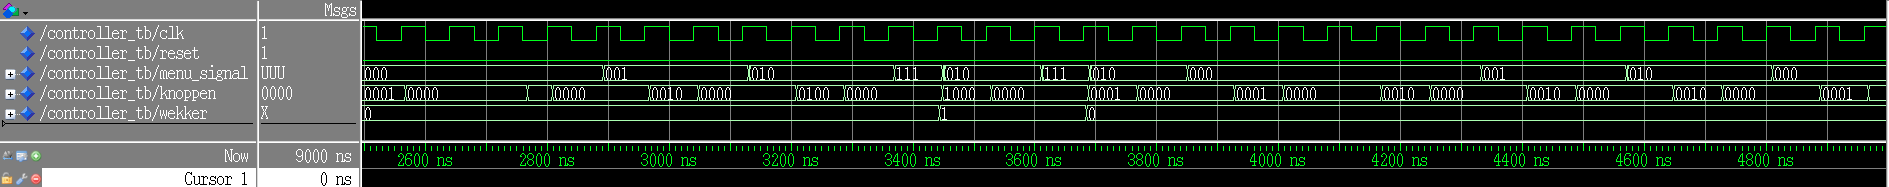
\includegraphics[width=\textwidth,height=\textheight,keepaspectratio]{Figuren/Controller/wave2_5-5_ext.png}
\caption{Simulatie van 2500ns tot 5000ns}
\label{fig:sim_ext_2_5-5}
\end{figure}
\begin{figure}[ht!]
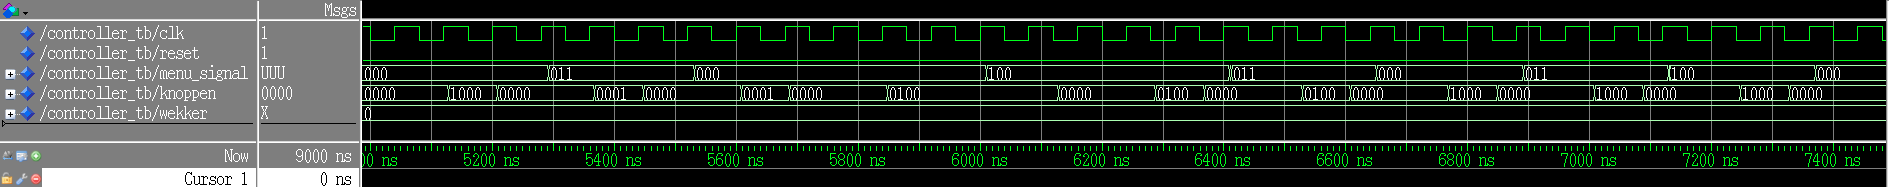
\includegraphics[width=\textwidth,height=\textheight,keepaspectratio]{Figuren/Controller/wave5-7_5_ext.png}
\caption{Simulatie van 5000ns tot 7500ns}
\label{fig:sim_ext_5-7_5}
\end{figure}
\begin{figure}[ht!]
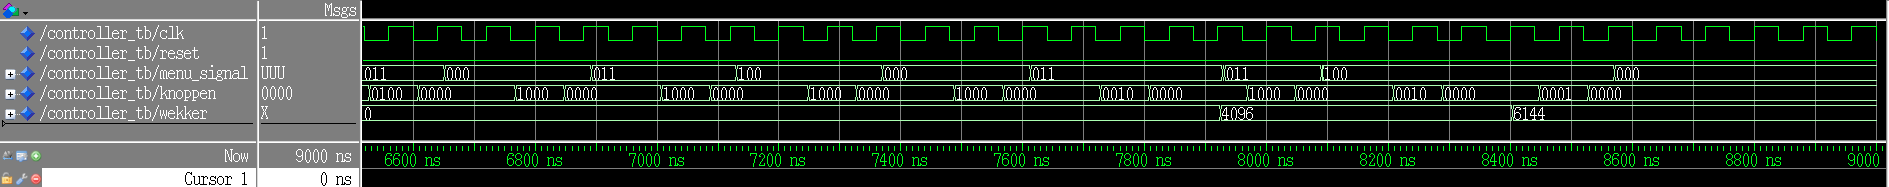
\includegraphics[width=\textwidth,height=\textheight,keepaspectratio]{Figuren/Controller/wave7_5-_ext.png}
\caption{Simulatie van 7500ns tot het einde}
\label{fig:sim_ext_7_5-}
\end{figure}
\newpage
\section{Timing}
\begin{figure}[ht!]
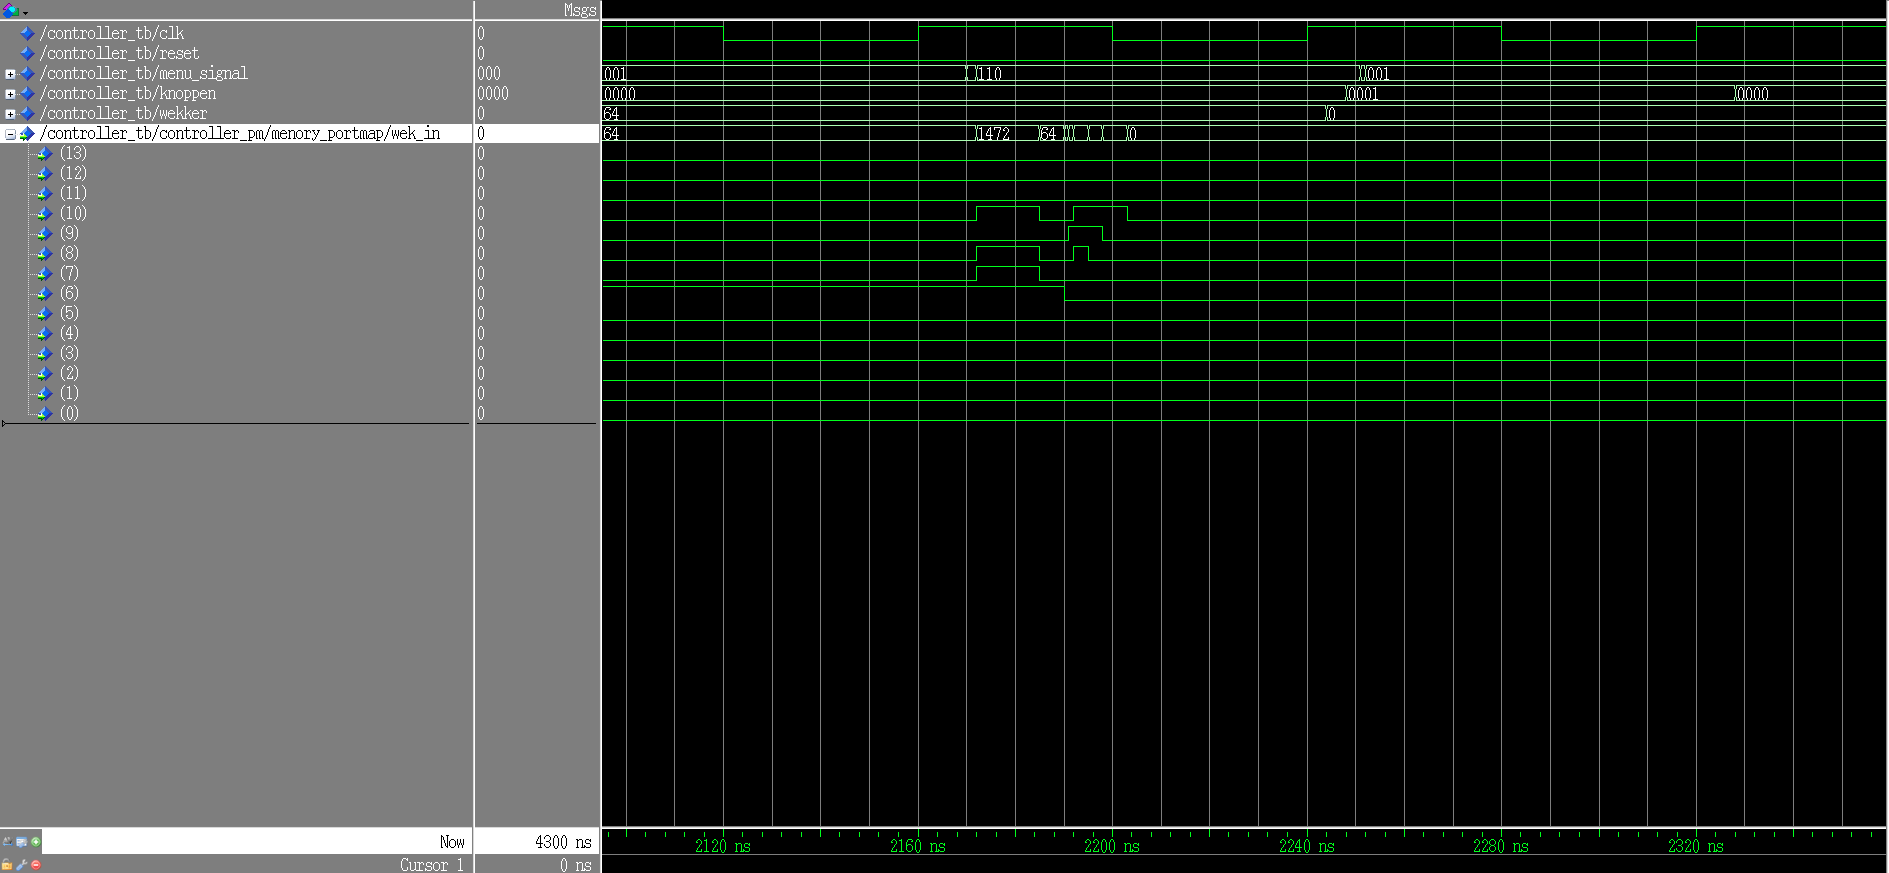
\includegraphics[width=\textwidth,height=\textheight,keepaspectratio]{Figuren/Controller/gliches_min.png}
\caption{Timing problemen}
\label{fig:timing_controller}
\end{figure}

\chapter[Simulatie resultaten Alarm]{Simulaties resultaten van het alarm}
\label{Ap:sim_alarm}
\section{Behavioral simulatie}
\begin{figure}[ht!]
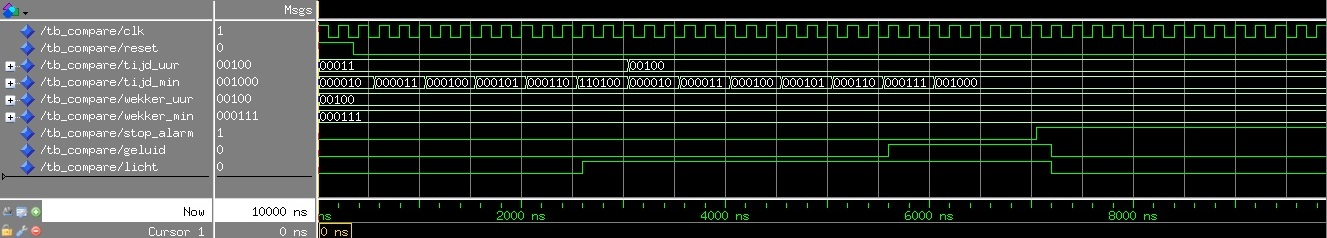
\includegraphics[width=\textwidth,height=\textheight,keepaspectratio]{Figuren/Alarm/Compare_beh.jpg}
\caption{Simulatie van 0 tot 10000 ns van compare}
\label{fig:sim_beh_compare}
\end{figure}
\begin{figure}[ht!]
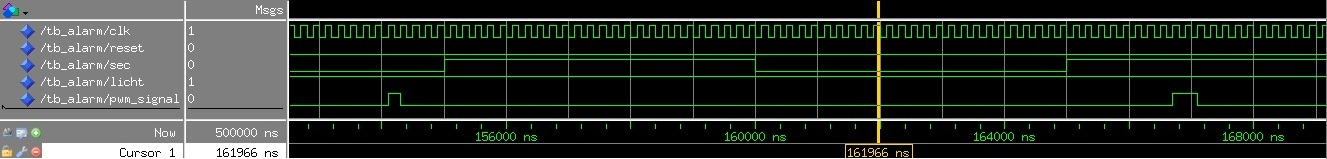
\includegraphics[width=\textwidth,height=\textheight,keepaspectratio]{Figuren/Alarm/Alarm_beh.jpg}
\caption{Simulatie van 151000 tot 170000 ns van alarm}
\label{fig:sim_beh_alarm}
\end{figure}
\newpage
\section{Extracted simulatie}
\begin{figure}[ht!]
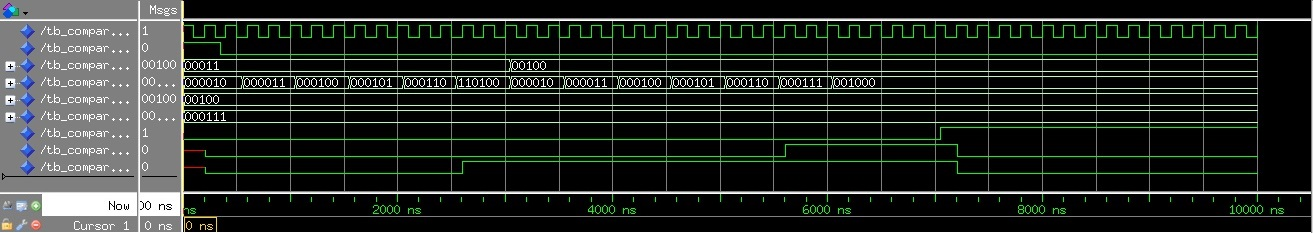
\includegraphics[width=\textwidth,height=\textheight,keepaspectratio]{Figuren/Alarm/Compare_ext.jpg}
\caption{Simulatie van 0 tot 10000 ns van alarm}
\label{fig:sim_ext_compare}
\end{figure}
\begin{figure}[ht!]
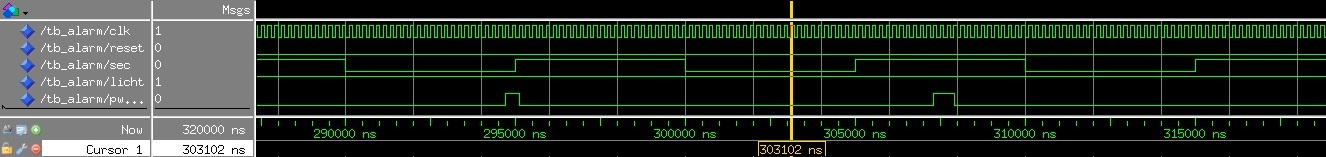
\includegraphics[width=\textwidth,height=\textheight,keepaspectratio]{Figuren/Alarm/Alarm_ext.jpg}
\caption{Simulatie van 290000 tot 320000 ns van alarm}
\label{fig:sim_ext_alarm}
\end{figure}

\chapter[Simulatie resultaten LCD]{Simulaties resultaten van het LCD}
\label{Ap:sim_LCD}
\section{Menu}
\begin{figure}[h!]
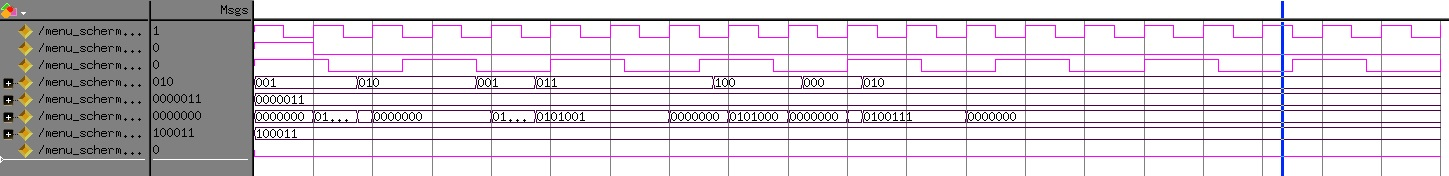
\includegraphics[width=\textwidth,height=\textheight,keepaspectratio]{Figuren/LCD/resultaten/menu.jpg}
\caption{Simulatie van het subblok menu}
\label{fig:simmenu}
\end{figure}
\section{Geluid}
\begin{figure}[h!]
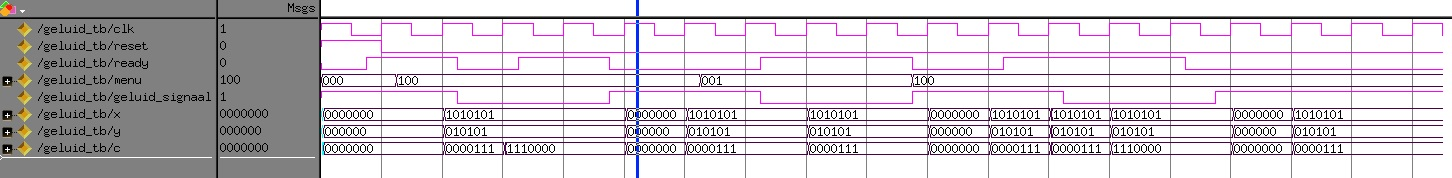
\includegraphics[width=\textwidth,height=\textheight,keepaspectratio]{Figuren/LCD/resultaten/geluid.jpg}
\caption{Simulatie van het subblok geluid}
\label{fig:simgeluid}
\end{figure}
\section{Licht}
\begin{figure}[h!]
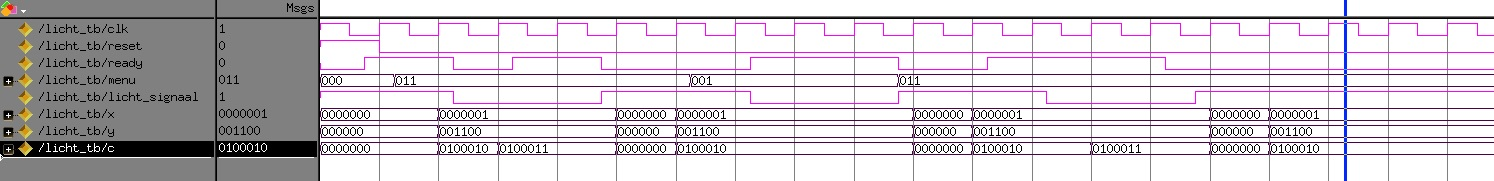
\includegraphics[width=\textwidth,height=\textheight,keepaspectratio]{Figuren/LCD/resultaten/licht.jpg}
\caption{Simulatie van het subblok licht}
\label{fig:simlicht}
\end{figure}
\section{DCF}
\begin{figure}[h!]
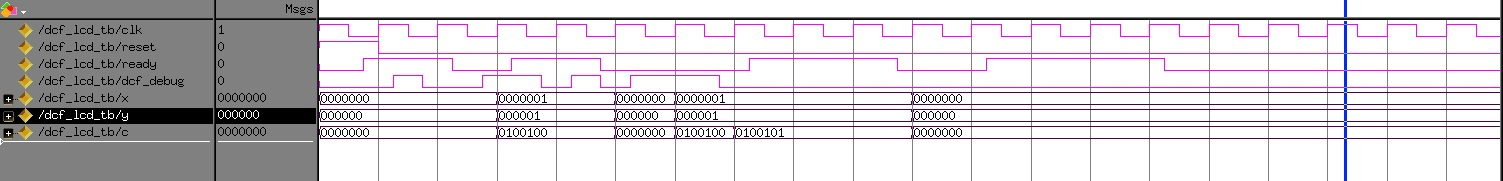
\includegraphics[width=\textwidth,height=\textheight,keepaspectratio]{Figuren/LCD/resultaten/dcf.jpg}
\caption{Simulatie van het subblok dcf}
\label{fig:simdcf}
\end{figure}

\begin{figure}[h!]
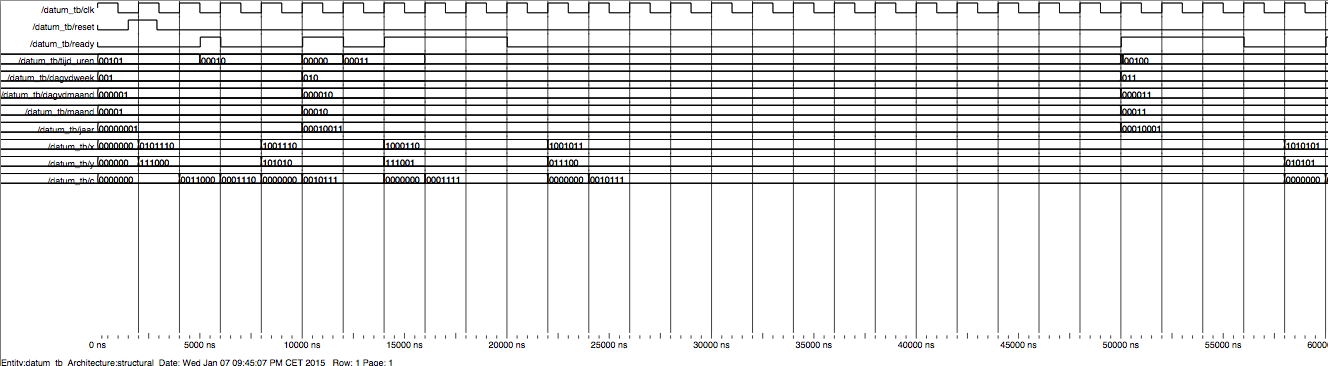
\includegraphics[width=\textwidth,height=\textheight,keepaspectratio]{Figuren/LCD/resultaten/simulatie_datum_behavioural.png}
\caption{Simulatie behavioural van het subblok datum}
\label{fig:sim_datum_behavioural}
\end{figure}

\begin{figure}[h!]
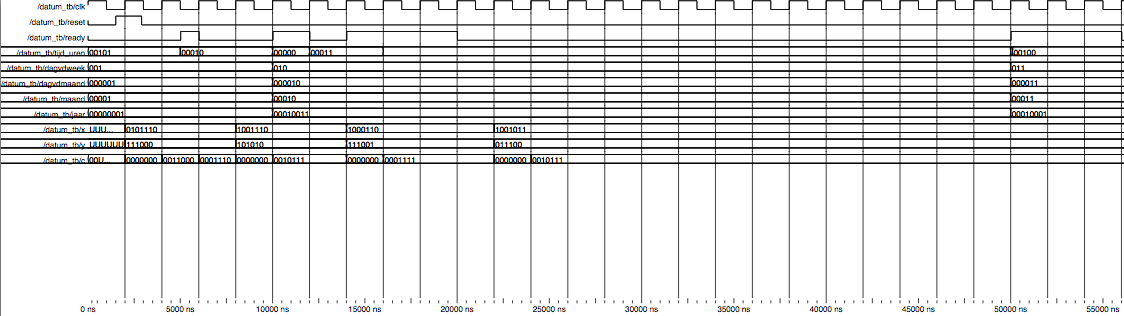
\includegraphics[width=\textwidth,height=\textheight,keepaspectratio]{Figuren/LCD/resultaten/simulatie_datum_circuit.png}
\caption{Simulatie circuit van het subblok datum}
\label{fig:sim_datum_circuit}
\end{figure}
